%%%%%%%%%%%%%%%%%%%%%%%%%%%%%%%%%%%%%%%%%
% Journal Article
% LaTeX Template
% Version 1.4 (15/5/16)
%
% This template has been downloaded from:
% http://www.LaTeXTemplates.com
%
% Original author:
% Frits Wenneker (http://www.howtotex.com) with extensive modifications by
% Vel (vel@LaTeXTemplates.com)
%
% License:
% CC BY-NC-SA 3.0 (http://creativecommons.org/licenses/by-nc-sa/3.0/)
%
%%%%%%%%%%%%%%%%%%%%%%%%%%%%%%%%%%%%%%%%%

%----------------------------------------------------------------------------------------
%	PACKAGES AND OTHER DOCUMENT CONFIGURATIONS
%----------------------------------------------------------------------------------------

\documentclass[twoside,twocolumn]{article}

\usepackage{blindtext} % Package to generate dummy text throughout this template 

\usepackage[sc]{mathpazo} % Use the Palatino font
\usepackage[T1]{fontenc} % Use 8-bit encoding that has 256 glyphs
\linespread{1.05} % Line spacing - Palatino needs more space between lines
\usepackage{microtype} % Slightly tweak font spacing for aesthetics

\usepackage[english]{babel} % Language hyphenation and typographical rules

\usepackage[hmarginratio=1:1,top=32mm,columnsep=20pt]{geometry} % Document margins
\usepackage[hang, small,labelfont=bf,up,textfont=it,up]{caption} % Custom captions under/above floats in tables or figures
\usepackage{booktabs} % Horizontal rules in tables

\usepackage{lettrine} % The lettrine is the first enlarged letter at the beginning of the text

\usepackage{enumitem} % Customized lists
\setlist[itemize]{noitemsep} % Make itemize lists more compact

\usepackage{abstract} % Allows abstract customization
\renewcommand{\abstractnamefont}{\normalfont\bfseries} % Set the "Abstract" text to bold
\renewcommand{\abstracttextfont}{\normalfont\small\itshape} % Set the abstract itself to small italic text

\usepackage{titlesec} % Allows customization of titles
\renewcommand\thesection{\Roman{section}} % Roman numerals for the sections
\renewcommand\thesubsection{\roman{subsection}} % roman numerals for subsections
\titleformat{\section}[block]{\large\scshape\centering}{\thesection.}{1em}{} % Change the look of the section titles
\titleformat{\subsection}[block]{\large}{\thesubsection.}{1em}{} % Change the look of the section titles

\usepackage{fancyhdr} % Headers and footers
\pagestyle{fancy} % All pages have headers and footers
\fancyhead{} % Blank out the default header
\fancyfoot{} % Blank out the default footer
\fancyhead[C]{Running title $\bullet$ May 2016 $\bullet$ Vol. XXI, No. 1} % Custom header text
\fancyfoot[RO,LE]{\thepage} % Custom footer text

\usepackage{titling} % Customizing the title section

\usepackage{hyperref} % For hyperlinks in the PDF

\usepackage{graphicx}

%----------------------------------------------------------------------------------------
%	TITLE SECTION
%----------------------------------------------------------------------------------------

\setlength{\droptitle}{-4\baselineskip} % Move the title up

\pretitle{\begin{center}\Huge\bfseries} % Article title formatting
\posttitle{\end{center}} % Article title closing formatting
\title{Article Title} % Article title
\author{%
\textsc{Frederik Vincent Primdahl} \textsc{Mikael Steenberg Pasovski} \and \textsc{Andreas Peter Brodersen} \textsc{Andreas Wede Gustavsen} \\[1ex] % Your name
\normalsize Copenhagen School of Design and Technology \\ % Your institution
%\and % Uncomment if 2 authors are required, duplicate these 4 lines if more
%\textsc{Jane Smith}\thanks{Corresponding author} \\[1ex] % Second author's name
%\normalsize University of Utah \\ % Second author's institution
%\normalsize \href{mailto:jane@smith.com}{jane@smith.com} % Second author's email address
}
\date{\today} % Leave empty to omit a date
\renewcommand{\maketitlehookd}{%
\begin{abstract}
\noindent \blindtext % Dummy abstract text - replace \blindtext with your abstract text
\end{abstract}
}

%----------------------------------------------------------------------------------------

\begin{document}

% Print the title
\maketitle

%----------------------------------------------------------------------------------------
%	ARTICLE CONTENTS
%----------------------------------------------------------------------------------------

\section{Introduction}
In the globalized economy of today, consumers are presented with a range of products to choose from when shopping. This can present some difficulty, as quality of the product is not always clear from its presentation. The customer review seeks to solve this by providing feedback on the purchase. Still, determining the value of a review can be difficult, as reviews can be misleading or provide little information.

Voting systems are often set in place to identify helpful reviews, and help consumers circumvent this issue, yet these reviews still get lost in the sheer number of unlabeled reviews. Our machine learning model aims to further filter reviews mainly by analyzing use of words, verbosity, among other aspects, to discover what makes a review helpful.

%------------------------------------------------
\section{Problem Formulation}

The main focus of this paper is to analyze Amazon review data across different categories and answer the question: “What makes an Amazon product review helpful?” through the use of classification models. In addition, answering “can you tell the helpfulness of a review based on name?”, “how does year affect the sentiment of the review?”

%------------------------------------------------
\section{Methods}

\subsection{Data exploration}

With the cleaned up dataset and the research question in mind*, columns with relevance are explored. To explore, we plot different columns of interest to identify any patterns in the data. We plot the distribution between reviews with votes and no votes as well as review rating.
\begin{figure}[h]
	\centering
	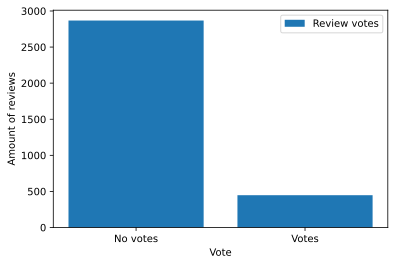
\includegraphics[width=0.5\textwidth]{img/no_votes_vs_votes.pdf}
	\caption{Vote distribution}
	\label{fig:votes_distribution}
\end{figure}
As seen in \figurename{\ref{fig:votes_distribution}}, the distribution is very uneven in favor of reviews with no votes. This is relevant when evaluating performance metrics of our model, as it indicates that a statistic like Youden's Index might be useful to counteract random guessing. To get another perspective on review votes we plot the data into a heatmap in relation to ratings.
\begin{figure}[h]
	\centering
	\includegraphics[width=0.5\textwidth]{img/rating_vote_heatmap_excluding_no_votes.pdf}
	\caption{Votes in relation to rating}
	\label{fig:rating_vote_heatmap}
\end{figure}
\figurename{\ref{fig:rating_vote_heatmap}} shows there is a drastic change after 11 upvotes. The reason could be that they dont see the need to upvote more when looking at upvotes combined with the rating, but this is nothing more than speculation.
\begin{figure}[h]
	\centering
	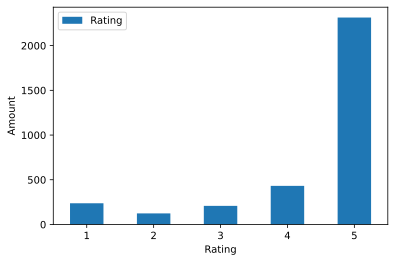
\includegraphics[width=0.5\textwidth]{img/rating_distribution.pdf}
	\caption{Rating Distribution}
	\label{fig:rating_distribution}
\end{figure}
Plotting the rating distribution, seen in \figurename{\ref{fig:rating_distribution}} we see a pattern that reviewers tend to give 5-star ratings. This might point to helpful reviews being of a more positive sentiment.
\begin{figure}[h]
	\centering
	\includegraphics[width=0.5\textwidth]{img/one_star_wordcloud.png}
	\caption{Common words used in 1-star reviews}
	\includegraphics[width=0.5\textwidth]{img/five_star_wordcloud.png}
	\caption{Common words used in 5-star reviews}
\end{figure}
Lastly we plot our review text into a wordcloud to get an overview of the differences between 1 and 5 star reviews


%------------------------------------------------

\section{Analysis}

\subsection{Data Preprocessing}
Initial data preparation was carried out on the whole dataset, dropping review time, image, style, ASIN, and reviewer id columns, as these were not needed. Unverified reviews were also filtered out, to avoid reviews from customers who did not purchase the product. Finally, null values were removed from the review text column.

As our input data mainly consists of unstructured text reviews, text normalization was done on the review text column to reduce randomness and reach a more uniform structure. This was done in accordance with common NLP data cleaning guidelines. Steps in this process involved removing non-word elements from the text – punctuation, symbols -, along with transforming each remaining word into lowercase. Because our model concerns itself with classification rather than sentiment, stop words like “not” did not provide any additional information to our model and were subsequently removed, as with other stop words contained in the NLTK “stopwords” library.

Each review was then tokenized into separate words using whitespace as a delimiter, as part of lemmatization to reduce morphological variation. Shortening some words to their root was thought important to improve model training efficiency. Lemmatization was chosen over stemming, as the accuracy of a lemmatizer in properly shortening words was more important than the speed of a stemmer.

As the final step of our data cleanup a column “voteSuccess” was added to the dataframe, calculating helpfulness of a review by dividing number of votes from the “votes”-column by quarters elapsed since the review was submitted. This was done to create a fairer indicator of helpfulness, since newer reviews would have had less time to accumulate helpfulness-votes and therefore appear less helpful.
%------------------------------------------------

\section{Findings}

\subsection{Subsection One}

A statement requiring citation \cite{Figueredo:2009dg}.
\blindtext % Dummy text

\subsection{Subsection Two}

\blindtext % Dummy text

%------------------------------------------------
\section{Conclusion}


%----------------------------------------------------------------------------------------
%	REFERENCE LIST
%----------------------------------------------------------------------------------------

\begin{thebibliography}{99} % Bibliography - this is intentionally simple in this template

	\bibitem[Figueredo and Wolf, 2009]{Figueredo:2009dg}
	Figueredo, A.~J. and Wolf, P. S.~A. (2009).
	\newblock Assortative pairing and life history strategy - a cross-cultural
	study.
	\newblock {\em Human Nature}, 20:317--330.

\end{thebibliography}

%----------------------------------------------------------------------------------------

\end{document}
